\documentclass[
    11pt,
]{article}

\usepackage{authblk}

% \usepackage{natbib}
% \setcitestyle{nature}

\usepackage[style=nature, natbib]{biblatex}

\addbibresource{References.bib}

\RequirePackage{luatex85, shellesc} % work around the LuaTex bug
% options for packages which may be loaded elsewhere
\PassOptionsToPackage{unicode=true, pdfa}{hyperref}
\PassOptionsToPackage{hyphens}{url}
\PassOptionsToPackage{dvipsnames,svgnames*,x11names*}{xcolor}

%==============================================================================%
%                                Load packages                                 %
%==============================================================================%

\usepackage{amsmath}                  % the AMS Math package - provides useful math environments and tools

\usepackage{amssymb}                  % provides useful symbols

\usepackage{amsfonts}                 % provides nice mathematical fonts

\usepackage{bm}                       % bold math

\usepackage{calc}                     % gives the ability to calculate in the document itself, inferior to but lighter weight than pythontex

\usepackage{cancel}                   % provides environments to cancel stuff in mathmode

\usepackage{esint}                    % better and more integral signs

\usepackage{enumitem}                 % enumerate and itemize improvements

\usepackage{fancyhdr}                 % fancy headers and footers

\usepackage[vario]{fancyref}          % for fancy cross-referencing with vario-style refs

\usepackage{graphicx}                 % facilitates inclusion of external graphics

\usepackage{parskip}                  % produces zero \parindent and non-zero \parskip

\usepackage{setspace}                 % set space between lines

\usepackage{xcolor}                   % colours bro

\usepackage{unicode-math}             % allows unicode characters in mathmode

\usepackage[pdfa, unicode]{hyperref}  % hyperlinks and PDF metadata manipulation

\usepackage{tikz}                     % drawing

\usepackage[siunitx]{circuitikz}      % drawing circuits

\usepackage{pgfplots}                 % plotting

\usepackage{geometry}                 % to set the margins of the page

\usepackage{subfig}

%==============================================================================%
%                             Set package options                              %
%==============================================================================%

%============================%
%          AMSMath           %
%============================%

\allowdisplaybreaks

%============================%
%          Hyperref          %
%============================%

\hypersetup{
    pdftitle={A minimal reaction-diffusion neural model generates C. elegans undulation},
    pdfauthor={Anshul Singhvi},
    colorlinks=true,
    linkcolor=Maroon,
    citecolor=Blue,
    urlcolor=Blue,
    breaklinks=true,
    pdfdisplaydoctitle = true
}

%============================%
%         Microtype          %
%============================%

% \UseMicrotypeSet[protrusion]{basicmath} % disable protrusion for tt fonts

%============================%
%     TikZ and PGFPlots      %
%============================%

\usetikzlibrary{
    arrows.meta,
    calc,
    decorations,
    decorations.pathreplacing,
    decorations.footprints,
    math,
    patterns,
    shadows,
    external
}

\tikzset{>=stealth}

\pgfplotsset{compat=1.16}

\usepgfplotslibrary{
    polar,
    colormaps,
    colorbrewer,
    groupplots,
    statistics
}

% This cycle list encodes the Wong colors, which are visually distinguishable.
% They also account for colorblind support, and as such are optimal for use in a paper.
\pgfplotscreateplotcyclelist{wong}{%
    color={rgb, 255 : red, 86  ; green, 180 ; blue, 233}, mark = *\\         % sky blue
    color={rgb, 255 : red, 230 ; green, 159 ; blue, 0},   mark = square*\\   % orange
    color={rgb, 255 : red, 0   ; green, 158 ; blue, 115}, mark = otimes*\\   % blueish green
    color={rgb, 255 : red, 240 ; green, 228 ; blue, 66},  mark = star\\      % yellow
    color={rgb, 255 : red, 0   ; green, 114 ; blue, 178}, mark = diamond*\\  % blue
    color={rgb, 255 : red, 213 ; green, 94  ; blue, 0},   mark = triangle*\\ % vermillion
    color={rgb, 255 : red, 204 ; green, 121 ; blue, 167}, mark = pentagon*\\ % reddish purple
}

\pgfplotsset{every axis legend/.append style={%
        cells={anchor=west}
    },
    cycle list name = wong,
}

%============================%
%          Geometry          %
%============================%

\geometry{
  a4paper,
  margin = 1.2in
}

%==============================================================================%
%                         Macros and document options                          %
%==============================================================================%

\setstretch{1} % line spacing of 1.25

\setlength{\emergencystretch}{3em}  % prevent overfull lines
\providecommand{\tightlist}{%
  \setlength{\itemsep}{0pt}\setlength{\parskip}{0pt}}
% \setcounter{secnumdepth}{0}
%
% % Redefines (sub)paragraphs to behave more like sections
% \ifx\paragraph\undefined\else
%     \let\oldparagraph\paragraph
%     \renewcommand{\paragraph}[1]{\oldparagraph{#1}\mbox{}}
% \fi
% \ifx\subparagraph\undefined\else
%     \let\oldsubparagraph\subparagraph
%     \renewcommand{\subparagraph}[1]{\oldsubparagraph{#1}\mbox{}}
% \fi

\newcommand{\inputtikz}[1]{%
  \tikzsetnextfilename{#1}%
  \input{#1.tikz}%
}

%==============================================================================%
%                            Neuron diagram macros                             %
%==============================================================================%

\newcommand{\doublec}[2]{% double diffusion arrows
  \draw  [-Circle] ($(#1.north east)!0.7!(#1.north)$) -- ($(#2.south east)!0.7!(#2.south)$);
  \draw  [Circle-] ($(#1.north west)!0.7!(#1.north)$) -- ($(#2.south west)!0.7!(#2.south)$);
  }

\newcommand{\singlec}[2]{% single diffusion arrows
  \draw [-Latex] (#1.east) -- (#2.west);
  }

% Set the TikZ neuron style up, since it's used many times
\tikzset{
  neuron/.style={
  % The shape:
  circle,
  % The size:
  minimum size=6mm,
  % The border:
  very thick,
  draw=blue!50!black!50,
  % The filling:
  top color=white,
  bottom color=blue!50!black!20, % and something else at the bottom
  % Font
  font=\itshape,
  % padding around node
  outer sep=2mm
  }
}


\tikzexternalize

\begin{document}
% \sffamily

%==============================================================================%
%                              Title and abstract                              %
%==============================================================================%

\title{A minimal reaction-diffusion neural model generates {\emph{C. elegans}} undulation}

\author[1]{Anshul Singhvi}

\author[1,3]{Harold Hastings}

\author[2]{Jenny Magnes}

\author[2]{Cheris Congo}

\author[2]{Miranda Hulsey-Vincent}

\author[1]{Rifah Tasnim}

\author[1]{Naol Negassa}

\affil[1]{Bard College at Simon's Rock}
\affil[2]{Vassar College}
\affil[3]{Hofstra University}

\date{\today}

\begin{abstract}
    The small (1 mm) nematode \emph{Caenorhabditis elegans} has become widely used as a model organism; in particular the \emph{C. elegans} connectome has been completely mapped, and \emph{C. elegans} locomotion has been widely studied (c.f. http://www.wormbook.org \citet{corsi2015}). We describe a minimal reaction-diffusion model for the \emph{C. elegans}, which results in similar behaviour to the neuromechanical model of \citet{izquierdo2018}. This  may be considered as a simple model for Xu et al.'s "descending pathway" description of the \emph{C. elegans} central pattern generator (CPG) \citet{xu2018,wen2012}. \citet{olivares2019} present a likely more realistic model which relies on small networks of neurons, and presents a distributed model of the CPG. In particular, we use simulation methods to show that a small network of \citet{fitzhugh1955}-\citet{nagumo1962} neurons (one of the simplest neuronal models) can generate key features of \emph{C. elegans} undulation (see \citet{magnes2012}), and thus locomotion.  Finally, we recreate the required oscillations and coupling with a network of coupled \citet{keener1983} analog neurons.
    % TODO: expand and inflate; fix grammar, cite Olivares2019
\end{abstract}

\maketitle

\section{Introduction}\label{sec: intro}

The small (1 mm) nematode \emph{Caenorhabditis elegans} (\emph{C. elegans}) has become widely used as a model organism \citep{corsi2015}, and has been among the most widely studied biological models of neuronal development, locomotion and the central pattern generator \citep{katz2016}.
The C. elegans connectome has been completely mapped \citep{jabr} and, as described below, its locomotion has been widely studied (\citet{corsi2015}).  There are a variety of neuronal models which can generate such undulation,
``When crawling on a solid surface, the nematode C. elegans moves forward by propagating sinusoidal dorso-ventral retrograde contraction waves.  A uniform propagating wave leads to motion that undulates about a straight line.'' \citep{kim2011}.
A different type of locomotion, often called swimming, occurs when nematodes are submerged in a liquid medium. The nematodes “switch” between these two gaits, under the regulation of particular serotonergic and dopaminergic neurons.

% TODO:
% - decide whether to cite CPG
% - italicise C. elegans
The purpose of this paper is to describe a minimal, biomimetic, reaction-diffusion model for the \emph{C. elegans} central pattern generator (CPG) \citep{xu2018, wen2012}.  We use simulation methods to show that a small network of \citet{fitzhugh1955}-\citet{nagumo1962} neurons (one of the simplest neuronal models) based on a skeleton model of the C. elegans CPG can reproduce key features of C. elegans undulation \citep{magnes2012} and thus locomotion.

In addition to simulating the CPG, we also implemented a modified version of the FitzHugh-Nagumo neuron, originally proposed by \citet{keener1983}, as an analog circuit.  This circuit solves the Keener differential equations, and we adjusted it to allow diffusive coupling between neurons.  We made a small network with these ``neuro-mimetic'' circuits, and showed that their behaviour replicates FitzHugh-Nagumo simulated behaviour.

% TODO - acknowledge prior work by Izquierdo et al.  May be more biologically relevant.  The role of this paper is to show a very minimal example.  We slightly modified the original FHN.

Olivares et al *** recently created a more biologically relevant model for the CPG, which argues that the CPG is a network of connected oscillators.  The role of this paper is to show a very minimal model, and our approach has been to create a small and computationally cheap model.

\section{The model central pattern generator}

% TODO show how the latest paper describes a small sequence of neurons forming coupled oscillators.

A central pattern generator is a small neural circuit which generates and regulates the movement of complex organisms.  This structure is present in different forms in many animals, and it regulates many types of periodic motion.  \citet{xu2018} proposed an architecture for the CPG of \emph{C. elegans} which is described below in \fref{fig: xu_cpg}.

In more complex animals, like horses or dogs, there is only one CPG; the dynamics of the CPG change depending on the gait of the animal \citep{collins1994}.  The mode of locomotion depends on the sequence in which the neurons fire, but the network's topology remains the same.  We show later that breaking the symmetry of the CPG model can lead to radical changes in behaviour.

\begin{figure}[h!]
    \label{fig: xu_cpg}
    \centering
    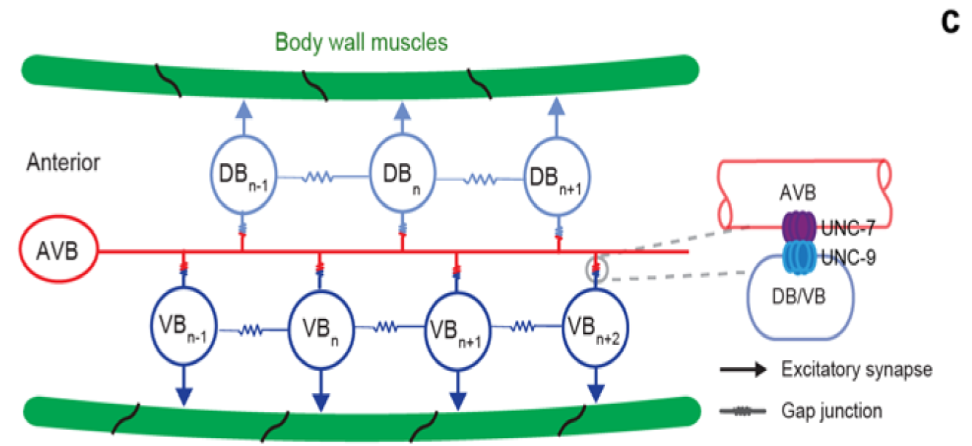
\includegraphics[width=9cm]{figures/xu_cpg/xu_cpg.png}
    \caption{The central pattern generator proposed by \citet{xu2018}.  Note the structure of the neurons, especially the head oscillator driving the descending pathway.}
\end{figure}

The central pattern generator has two principal components.  First is the \textbf{head oscillator}. As described by \citet{gjorgjieva2014}, the head oscillator consists of two “head neurons” with mutually inhibitory coupling.  Oscillations are generated when this coupling destabilizes an excitable steady state.

In the terms of dynamical systems analysis, the oscillations destabilize to a stable limit cycle.  The mutual inhibition and symmetry between neuron pairs leads to a phase lock of $180^\circ$.  This provides out-of-phase stimuli which propagate through the descending pathway, with the inhibition between neuron pairs keeping the oscillations stable.
% TODO experiment on a single head oscillator.
% TODO explain how coupling works

Second is the \textbf{descending pathway}, which consists of pairs of coupled, excitable, dorsal and ventral neurons.  These follow the body of the worm, and are linked to motor neurons and muscles.  The head oscillator drives the descending pathway, and the pathway is kept in sync by mutual inhibitory coupling between neurons.

% TODO do we need this?
% One can think of the CPG as a driven, dissipative system.  An analogy to the driven, damped oscillator is particularly apt - in the CPG, the head oscillator drives the descending pathway.

% TODO expand.  Our model could have had more neurons, with a shorter phase lag between pairs.
While \textit{C. elegans} has twelve pairs of motor neurons, we have only used six pairs in our model.  \Fref{fig: cpg} is a depiction of our simplified model as a graph, wherein neurons are nodes, and the arrows between them symbolize connections.

\begin{figure}[h!]
    \label{fig: cpg}
    \centering
    \inputtikz{figures/cpg/cpg}
    \caption{Our simplified central pattern generator model.  Descending coupling (shows inhibitory connections, and potential flows through gap junctions, not necessarily symmetric)}
\end{figure} % TODO: legend

\section{The FitzHugh-Nagumo Neuronal Model}\label{sec: fhn}

In accord with the goal of this paper, we sought the simplest relevant neuronal model.  The classical Hodgkin-Huxley\cite{hodgkin1952} model of squid neurons has led to a variety of simpler conduction models, including the Morris-Lecar\cite{morris1981} and Fitzhugh-Nagumo (FHN) models.

The FHN model consists of two dynamical variables; a fast activator variable $v$ corresponding to the (rescaled) membrane potential, and a slow inhibitor variable $w$ corresponding to a generalized gating variable.

\begin{equation}
    \label{eq: fhn}
    \begin{aligned}
        dv &= f(v) + w - I_\mathrm{ext}\\
        dw &= \epsilon (a - bv)\\
        f(v) &= \frac{v^3}{3} - v
    \end{aligned}
\end{equation}

The parameter $I_\mathrm{ext}$ is an external driving current, and can also be used to increase excitability.  In the analog implementation, this is an integral component of tuning the neuron's frequency response.

In this system, $f(v)$ can be any function which retains the appropriate dynamics, in that it has the same general shape as the cubic $f(v)$.  In our analog implementation, we use a piecewise linear approximation to the cubic, in order to simplify the circuit and avoid using expensive components.  Here, the position of the $w$-nullcline is controlled by $a$, and the vertical translation of the $v$-nullcline is controlled by $I_{ext}$

Xu et al. used a simplified two-variable model consisting of a fast, cubic-like activator variable (see the V-nullcline) and a slow, non-linear inhibitor variable (see the n-nullcline). The Fitzhugh-Nagumo model has similar activator nullclines.

% TODO: remove Morris-Lecar
% remark that if the w and v nullclines come near each other, you see a critical slowdown.
% In Hodgkin-Huxley notation, $n$ is the potassium channel.  In the FHN formulation, this corresponds to the $w$ gate variable.
\begin{figure}[h!]
    \label{fig: nm nullclines}
    \centering
    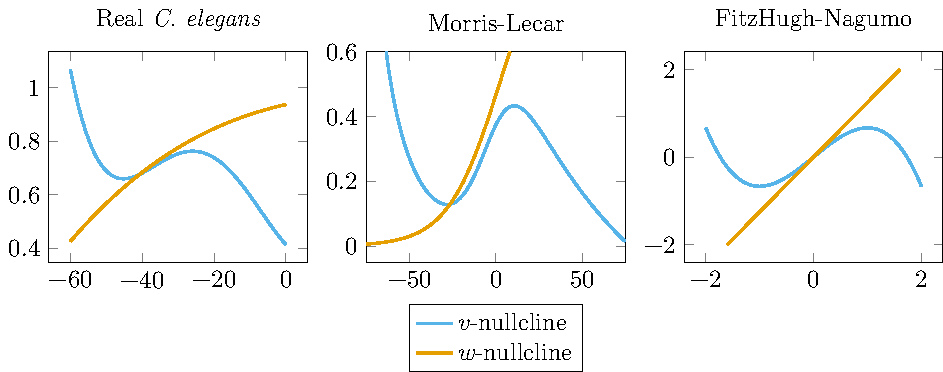
\includegraphics{figures/neuron_dynamics/neuron_dynamics.pdf}
    % note that in the vicinity of the v-nullcline, the w-nullcline is essentially straight.
    \caption{Nullclines of several different neuronal models; on the right is the biological model of Xu et al, in the centre is the Morris-Lecar model, and to the right is the FitzHugh-Nagumo model.  These have been arranged in order of decreasing complexity.}
\end{figure}

% TODO: see if anyone else used diffusion to couple neurons
The original system was meant to model one neuron only.  Following ***, we used
generalized diffusion coupling between FHN neurons to mimic synapses.
A positive coefficient would simulate a gap junction, or
an excitatory synapse; a negative coefficient would simulate inhibitory
coupling (\citet{collins1994}).

% TODO: there will be other examples...cf them

The equations, when modified for synaptic connections, look like this:

\begin{equation}
    \label{eq: fhnd}
    \begin{aligned}
        dv   &= f(v) + w - I_\mathrm{ext} + \color{green}{D(Δv)}\\
        dw   &= ϵ(a - bv)\\
        f(v) &= \frac{v^3}{3} - v
    \end{aligned}
\end{equation}

where $\Delta v$ is the difference in voltage between the driving and driven neurons, essentially $\Delta v = v_{driven} - v_{driving}$.

\begin{figure}[h!]
    \label{fig: fhn_dynamics}
    \centering
    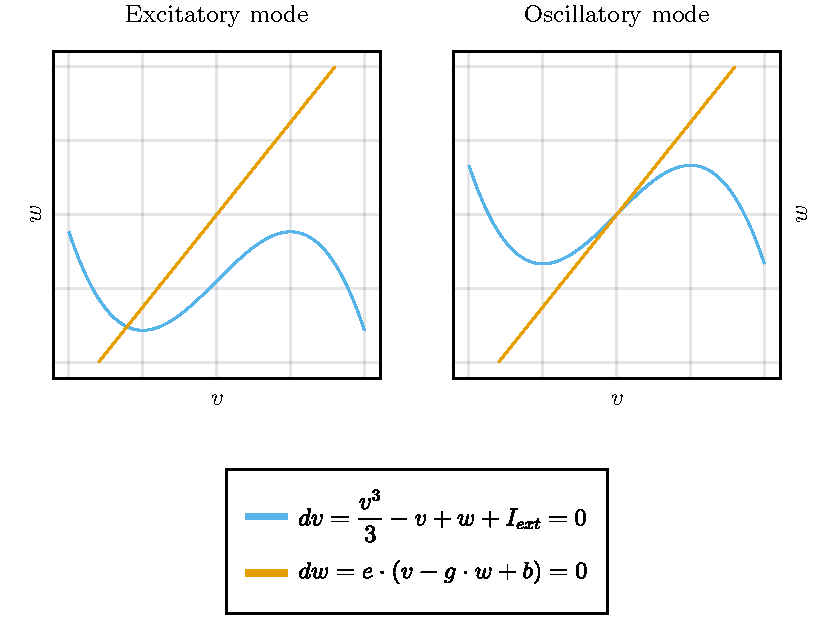
\includegraphics{figures/fhn_dynamics/fhn_dynamics.pdf}
    \caption{The nullclines of the FitzHugh-Nagumo neuron.  Nullclines are isoclines where the derivative of a variable is zero.  Here we show an oscillatory mode and an excitable one.  In an oscillating cell, the stable equilibrium is replaced by an unstable equilibrium (open circle) around which it circles indefinitely.  See \citet{parsons2018} for a clear explanation of the dynamics of oscillatory biological systems.}
\end{figure} % TODO: legend



\section{Simulation}

We performed the simulations in Python, using the standard SciPy ODE solvers, which wrap LSODA. % TODO list solver here

\subsection{Methods}

See the appendix, or attached code, for how we simulated this motion.  It will be published on Github with embedded plots, so people can see it.

We realize the network shown in \Fref{fig: cpg} into a system of ODEs, and solve it.  The equations are integrated, giving a timeseries of neuronal potentials.  These were passed through filters to simulate muscular movement and the resistance of the medium.  We used Gaussian smoothing and B-splines for this purpose.
% TODO: reference for muscle response time

We generated a video by fixing the head of a worm to the origin, and re-normalizing the coordinates resulting from the filtering.

\subsection{Comparison to real worm}

Cite the paper which Jenny sent here.  It can be seen that our model closely approximates an unconstrained worm, specifically of the wild type.

While the angle which a worm crawling on agar subtends tends to be oblique, as the constraint on the worm decreases, the angle becomes more and more acute - consider the videos.  It is not hard to see that a fully unconstrained worm might behave much like our model does.

The worm generates sinusoidal oscillations

% Closely related to the first I&B (2008).  Alternate and likely more realistic structure with a distributed CPG was proposed by new Izquierdo.

\section{Analog implementation}

\citet{nagumo1962} proposed a circuit to simulate a FitzHugh-Nagumo neuron, shown in \Fref{fig: nagumo_ckt}.  It used a tunnel diode to achieve a cubic-like activation function, and an inductor to differentiate the K current.  However, this approach presents several complications.  Tunnel diodes are rare, and rather expensive; inductors cannot be used in proximity because of mutual inductance effects, and are quite large.

\begin{figure}[h!]
    \centering
    \inputtikz{figures/nagumo/nagumo}
    \caption{The original circuit proposed by \citet{nagumo1962}.  Note the use of inductors for differentiation, and the tunnel diode to supply a cubic-like V-I curve.  Our circuit, based off \citet{keener1983}, is arranged in the same layout, to make the similarities and differences more explicit.}
    \label{fig: nagumo_ckt}
\end{figure}

% The circuit in \Fref{fig: nagumo_ckt} is an analog solver for the FitzHugh-Nagumo equations.  Namely, the

The sodium channel in the FitzHugh-Nagumo equations has a negative resistance regime, wherein the current decreases as the voltage increases.  Nagumo's tunnel diode exhibits this behaviour, but it may be replaced by any device with a similarly nonlinear V-I curve.  The necessary feature is that in the oscillatory regime, the system is a relaxation oscillator, and that it has an excitable regime.

\citet{keener1983} proposed a modified Nagumo circuit which used the saturation properties of operational amplifiers ("op-amps") to achieve cubic-like non-linearity in the FHN model. He also used an op-amp and a capacitor to simulate the inductor in the original Nagumo circuit.

As a result of the piecewise linear approximation to the cubic, the nullclines of the circuit system differ slightly from the original FitzHugh-Nagumo nullclines.  However, in experiments this did not cause a significant change in the dynamics of the individual neuron, or many connected together - the nullclines are sufficiently similar that the dynamics are effectively the same.

Our modifications to Keener's proposed circuit are mainly concerned with diffusive coupling between neurons.  If each individual circuit is thought of as a single neuron, then we implemented diffusive coupling methods between those neurons.  We also found that you don't need separate power supplies, and you can get finer control by adjusting the bias voltage and input through a separate mechanism.

\begin{figure}[h!]
    \centering
    \inputtikz{figures/neuron_unit/neuron_unit}
    \caption{The circuit we created, based of \citet{keener1983}.  Note the use of operational amplifiers in place of the inductor and tunnel diode; though this circuit looks more complex, in practice it is quite simple to implement.}
    \label{fig: neuron_unit}
\end{figure}

However, this is only one neuron.  In order to implement a full central pattern generator, we implemented diffusive coupling mechanisms.  These mechanisms are shown in \Fref{fig: coupling_ckt}.  We implemented a positive diffusion coefficient by passing the voltage through a resistor (to simulate $D$), and then a diode (to simulate $\mathrm{max}(\Delta v, 0)$).  The negative diffusion coefficient was implemented by using an inverting amplifier with a small gain, and then passing through a diode.
\newsavebox{\tempbox}
\begin{figure}
    \centering
    \inputtikz{figures/coupling/coupling}
    \caption{Coupling methods}
    \label{fig: coupling}
\end{figure}

\subsection{Comparison of analog and simulation}

To compare the analog implementation with our simulated model, we will focus on the timeseries output of the neurons, and not on the end worm.  Include the relevant figure here - you can see clearly that the effect is the same.  There are some differences in the waveform because of the different activation function in the circuit (linear interpolation).

\begin{figure}[h!]
    \centering
    \pgfplotsset{}
    % \inputtikz{figures/anal_sim_comp/anal_sim_comp}
    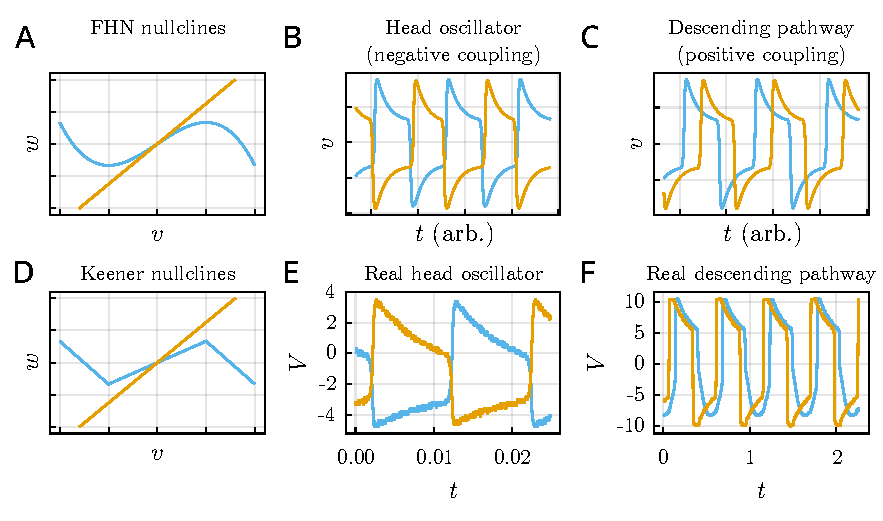
\includegraphics{figures/anal_sim_comp/anal_sim_comp}
    \caption{Comparison between simulated dynamics (top row) and observed dynamics in circuit (bottom row).}
    \label{fig: anal_sim_comp}
\end{figure}

% TODO: write up a section on the Beer paper and see how it relates to our CPG model.
% Perhaps a discussion about the "scientific lineage" of our model, and the Olivares et al model.
% Paraphrase their description.

\section{Conclusion}

Mention the bullet points from the presentation.  How could a system like this be used in applications?  End with some future paths.

We have shown that the undulatory motion of \emph{C. elegans} can be simulated using a structured central pattern generator, and simple, biomimetic neurons.  This system is computationally cheap, and translates to a simple analog circuit.

Our model of the nematode is surprisingly similar to real unconstrained motion.  While most measurements of \emph{C. elegans} are taken on horizontal agar sheets, observations made in clear, water-filled cuvettes where the worm floats freely seem to resemble our simulated worm more.

Given the flexibility of the model, by introducing defects and asymmetries into the topology, we can study how mutations affect the nematode's motion, as well as the structures underlying differences in phenotypes.

% The particular model doesn't really matter; if you have the right topology, you can generate the behaviour.
% Reservoir computing and our neurons.  Speculate that different circuits of FHN neurons might be suitable dynamical reservoirs.  However, a CPG has a range of comparatively simple dynamics.
% cite Sanchez-Sinencio, Spano on circuits.  Theirs emphasize accuracy whereas ours emphasizes speed and minimal cost.

Reference some connections to \citet{adamatzky2008} - the neural system as a computational system.  Also cite similarity between B-Z and FHN.

\section{References}

% \nocite{*}
% \bibliography{References}
\printbibliography[heading=none]
\end{document}
